\documentclass[../main.tex]{subfiles}

\begin{document}
\section{Conics in a nutshell}
In this section will revise some basic properties of conics, that will be used in the next sections for the study of the motion of two bodies under the influence of gravity.
\subsection{General conics}
\begin{definition}
  A conic is the curve obtained as the intersection of a plane with the surface of a double cone (a cone with two \emph{nappes}).
\end{definition}
In \cref{fig:conics} we show the 3 types of conics: the ellipse, the parabola, and the hyperbola, which differ on their eccentricity, as we will see later on. Note that the circle is a special case of the ellipse.
\begin{figure}[htbp]
  \centering
  \begin{minipage}[ht]{0.45\textwidth}
    \centering
    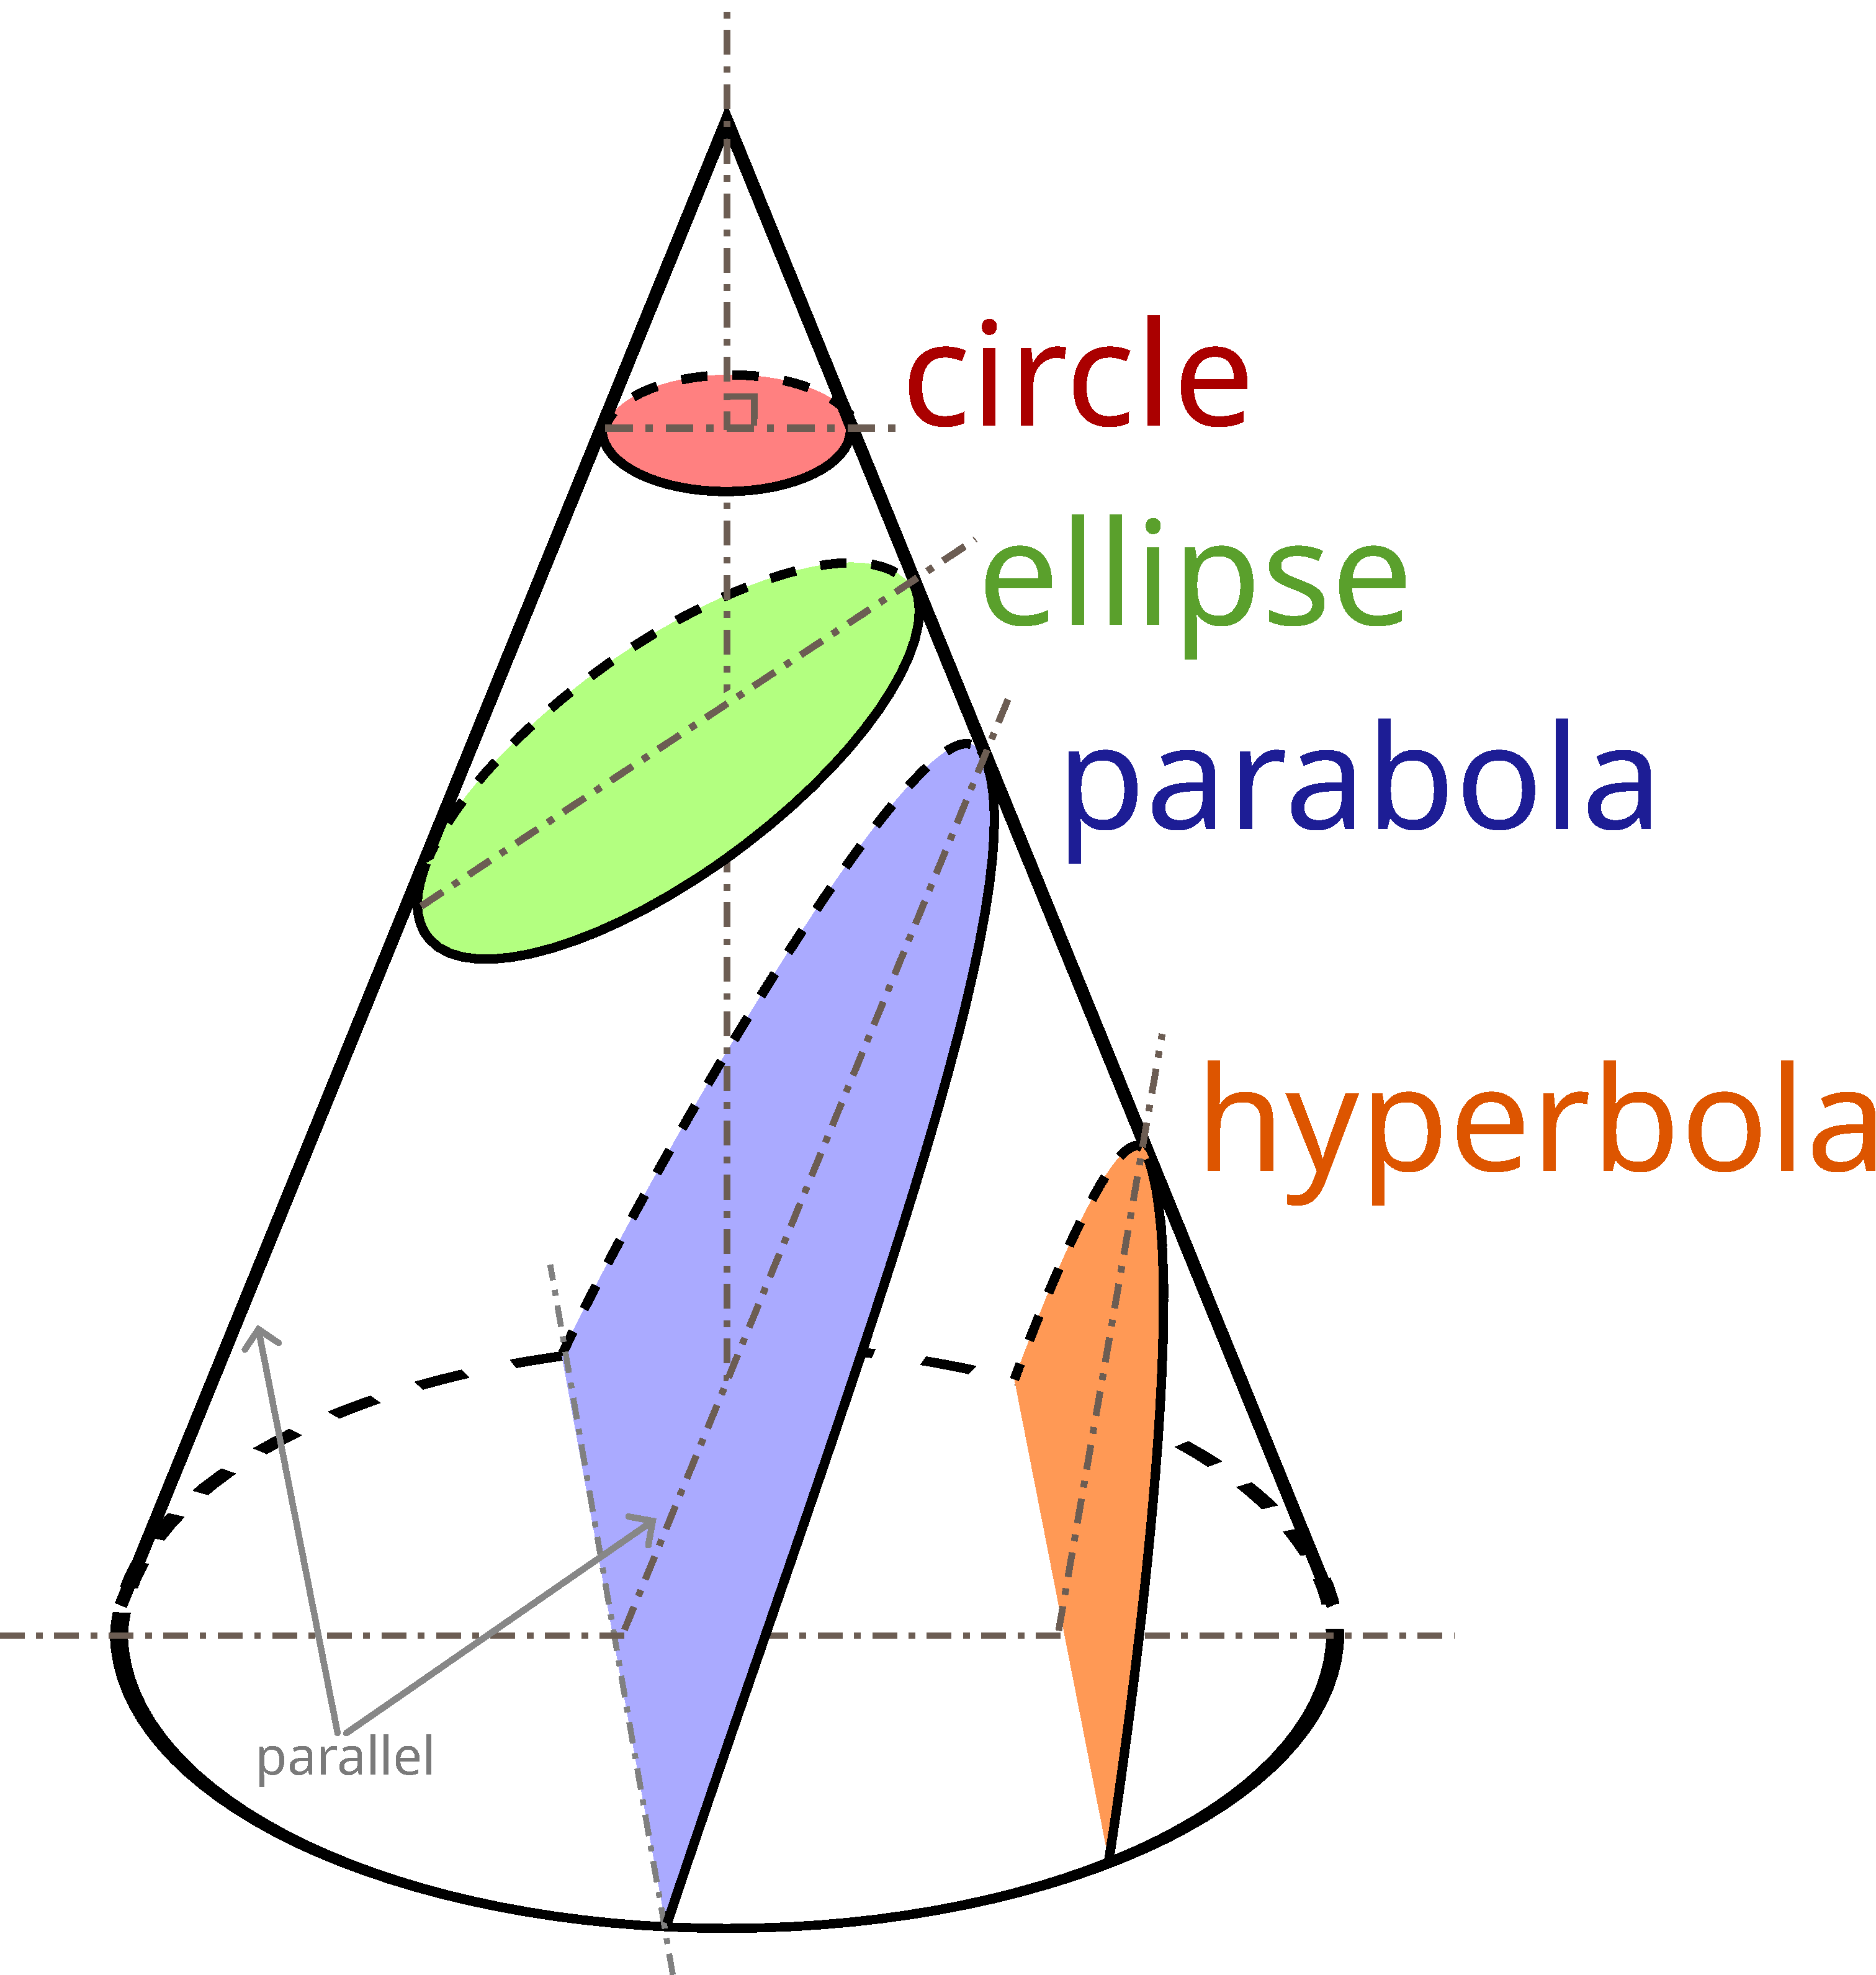
\includegraphics[width=\textwidth]{Images/Conic_Sections.pdf}
    \caption{The black boundaries of the colored regions are conic sections. The other half of the hyperbola, which is not shown, is in the other nappe of the double cone. Source: \cite{wiki:conic}.}
    \label{fig:conics}
  \end{minipage}
  \hspace{0.0333333\textwidth}
  \begin{minipage}[ht]{0.45\textwidth}
    \centering
    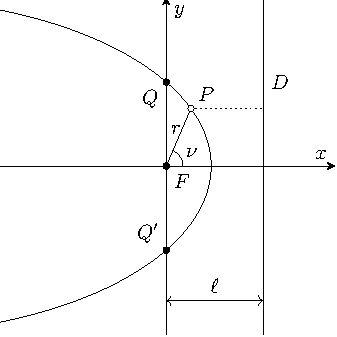
\includegraphics[width=\textwidth]{Images/conics.pdf}
    \caption{Reference frame centered at the focus of the conic and whose axes are such that the $y$-axis is parallel to the directrix and the $x$-axis is perpendicular to the directrix. The directions of the axes are chosen arbitrarily, subject to the constraint that a right-handed system $(x,y)$ is obtained.}
    \label{fig:conics_cartesian}
  \end{minipage}
\end{figure}
The following proposition gives a characterization of the conics.
\begin{proposition}
  A conic is the set of all points $P$ such that the distance from $P$ to a fixed point $F$ is a multiple of the distance from $P$ to a fixed line $D$. Mathematically, this is expressed as:
  \begin{equation}\label{eq:conic_pre}
    d(P,F)=e d(P,D)
  \end{equation}
  where $d$ is the Euclidean distance. The point $F$ is called \emph{focus}; the line $D$, \emph{directrix}, and the constant of proportionality $e$, \emph{eccentricity}.
\end{proposition}
An important type of conic section is when $e=0$, but this definition is not valid in this case, as it reduces to a single point. In this case, the conic obtained, a \emph{circle}, is defined as the set of all points $P$ such that the distance from $P$ to a fixed point $F$ is constant. It can be thought as a limit case of \cref{eq:conic_pre} by letting the line $D$ to infinity in a specific rate.

Note that using the polar coordinates $(r,\nu)$ centered at $F$ (as in \cref{fig:conics_cartesian}), we can rewrite \cref{eq:conic_pre} as:
\begin{equation}\label{eq:conic}
  r=e(\ell - r\cos\nu)\implies r= \frac{e\ell}{1+e\cos\nu}=:\frac{p}{1+e\cos\nu}
\end{equation}
where we have defined $p:=e\ell$.
\begin{definition}
  Let $C$ be a conic and $e$ be its eccentricity. We say that $C$ is
  \begin{itemize}
    \item an \emph{ellipse} if $0\leq e<1$.
    \item a \emph{parabola} if $e=1$.
    \item a \emph{hyperbola} if $e>1$.
  \end{itemize}
  If $e=0$, the conic is called \emph{circle}.
\end{definition}
\subsection{Ellipse}\label{sec:ellipse}
From now on we will focus on the study of the ellipse. From \cref{eq:conic}, since $e<1$, it follows that $r(\nu)$ is continuous, $2\pi$-periodic and satisfies $r(0)=r(2\pi)$. Therefore, the ellipse is a bounded and closed curve, and it is the only conic section satisfying these two properties.

Let's now study the extrema of $r(\nu)$. An easy check shows that the minimum is attained at $\nu=0$ and the maximum at $\nu=\pi$ and these values are given by:
\begin{equation}
  r_\mathrm{min}=\frac{p}{1+e}\qquad\text{and}\qquad r_\mathrm{max}=\frac{p}{1-e}
\end{equation}
When considering orbits of celestial bodies these points are called \emph{periapsis} and \emph{apoapsis}, respectively\footnote{Other names are used in the literature when the central body and the orbiter are particular ones. For example for the system Sun-Earth, the words \emph{perihelion} and \emph{aphelion} are used, whereas for the system Earth-Moon, the words \emph{perigee} and \emph{apogee} are used instead.}. The line connecting both points is called \emph{line of apsides}. Let's seek now the extrema of $x = r\cos\nu$ and $y = r\sin\nu$. Differentiating with respect to $\nu$ yields:
\begin{equation}
  x'=-\frac{p\sin\nu}{{(1+e\cos\nu)}^2}\qquad y'=\frac{p(e+\cos\nu)}{{(1+e\cos\nu)}^2}
\end{equation}
On the one hand, the former expression vanishes at $\nu=0,\pi$. Therefore, the extrema of $x$ coincide with the periapsis and apoapsis points and at these points the $y$ coordinate is equal to 0. This means that the line of apsides passes through the focus of the ellipse. On the other hand, $y'$ vanishes at $\cos\nu=-e$. That is, at $\nu=\arccos (-e)$ and $\nu=2\pi-\arccos(-e)$. Therefore, using that $\sin(\arccos x)=\sqrt{1-x^2}$, the values of $y$ at these extrema are:
\begin{equation}
  y_\mathrm{min}=\frac{p}{1-e^2}\sin(2\pi-\arccos(-e))=-\frac{p}{\sqrt{1-e^2}}\qquad y_\mathrm{max}=\frac{p}{1-e^2}\sin(\arccos(-e))=\frac{p}{\sqrt{1-e^2}}
\end{equation}
Note that the $x$ coordinate at these two points is the same: $\displaystyle-\frac{pe}{1-e^2}$.
\begin{definition}
  Consider the reference frame of \cref{fig:ellipse} centered at one focus. We define the \emph{semi-major axis} $a$ as half the segment that connects the two extrema of the $x$ coordinate. The \emph{semi-minor axis} $b$ is defined as half the segment that connects the two extrema of the $y$ coordinate. The length of those segments are also denoted by $a$ and $b$, respectively. Thus, these are given by the following expressions:
  \begin{equation}
    a:=\frac{x_\mathrm{max}-x_\mathrm{min}}{2}=\frac{r_\mathrm{max}+r_\mathrm{min}}{2}=\frac{p}{1-e^2}\qquad b:=\frac{y_\mathrm{max}-y_\mathrm{min}}{2}=\frac{p}{\sqrt{1-e^2}}
  \end{equation}
\end{definition}
\begin{figure}[htbp]
  \centering
  \begin{minipage}[ht]{0.47\textwidth}
    \centering
    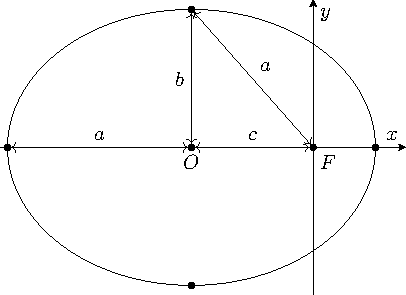
\includegraphics[width=\textwidth]{Images/ellipse.pdf}
    \caption{Ellipse}
    \label{fig:ellipse}
  \end{minipage}
  \hspace{0.02\textwidth}
  \begin{minipage}[ht]{0.47\textwidth}
    \centering
    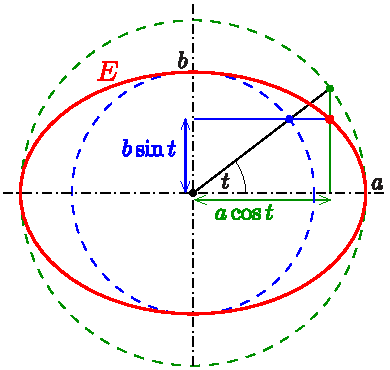
\includegraphics[width=\textwidth]{Images/circles-ellipse.pdf}
    \caption{Reference frame centered at the center of the ellipse. Source: \cite{wiki:conic-ellipse}.}
    \label{fig:circle-ellipse}
  \end{minipage}
\end{figure}
\begin{figure}[ht]

\end{figure}
From here note that we can express $b$ in terms of $a$ and $e$ as:
\begin{equation}\label{eq:ellipse_b_a}
  b=a\sqrt{1-e^2}
\end{equation}
\begin{definition}
  We define the center of the ellipse $O$ as the intersection of the semi-major axis and semi-minor axis. The \emph{linear eccentricity} $c$ is defined as the distance between the center $O$ and the focus $F$.
\end{definition}
We have just found a relation between $a$ and $b$. Now, we would like to find a similar relation between $a$ and $c$. To do so, let's calculate the distance from the focus $F$ to one of the extrema of the $y$ coordinate.
\begin{equation}
  d\left(F,\left(-\frac{pe}{1-e^2},\pm \frac{p}{\sqrt{1-e^2}}\right)\right)=\frac{p}{\sqrt{1-e^2}}\sqrt{\frac{e^2}{1-e^2}+1}=\frac{p}{1-e^2}=a
\end{equation}
Hence, the value of $c$ can be simplified to (see \cref{fig:ellipse}):
\begin{equation}
  c^2=a^2-b^2=a^2-a^2(1-e^2)=a^2e^2\implies c=ae
\end{equation}
Finally, one more property of the ellipse will be needed: its area.
\begin{proposition}
  The area enclosed in an ellipse of semi-major axis $a$ and semi-minor axis $b$ is $\pi a b$.
\end{proposition}
\begin{proof}
  Consider the ellipse $E$ centered at the origin and oriented as in \cref{fig:circle-ellipse}. From \cref{fig:circle-ellipse} one can check that it can be parametrized by $(x,y)=(a\cos t,b\sin t)$ with $ t\in[0,2\pi)$. This parametrization satisfies:
  \begin{equation}
    \frac{x^2}{a^2}+\frac{y^2}{b^2}=1
  \end{equation}
  Hence, the area enclosed in the ellipse is can be parametrized by $(x, y)=(ar\cos t,br\sin t)$, with $r\in[0,1]$ and $t\in[0,2\pi)$. The Jacobian of this transformation is $abr$. Therefore, from the change of variable theorem we have that:
  \begin{equation}
    \mathrm{Area}(E)=\iint_E\dd{x}\dd{y}=\int_{0}^{2\pi}\int_{0}^{1}abr\dd{r}\dd{t}=\pi ab
  \end{equation}
\end{proof}

\end{document}